\documentclass[UTF8]{ctexart}
\usepackage{graphicx}
\usepackage{float}
\usepackage{ragged2e}
\usepackage{amsthm}
\usepackage{tikz}
\usetikzlibrary{arrows.meta}
\newtheorem{problem}{题}
\newtheorem{solution}{解}
\usepackage{amssymb}
\usepackage{amsmath}
\usepackage{wrapfig}
\usepackage{hyperref}
%\newcommand{\mathrm{d}}{\mathrm{d}}
%\newcommand{\mathrm{i}}{\mathrm{i}}

\title{答案}
\author{limbo137}
\begin{document}
\maketitle
\subsection{简谐振动}
这是复数的第一个重要应用,在简谐运动中,质点运动遵循的方程是
\[\ddot{x} = -\omega^2 x\]
首先按照一般的解方程的套路,我们往往会设
\[x = Ce^{at}\]
代入,得
\[a^2 = -\omega^2\]
从这个方程就可以得到
\[a = \pm \mathrm{i} \omega\]
之后的操作就是把$a$带回去,得到两个线性无关特解,但是我们今天要用另一种方式来解这个方程

我们首先设$\omega u=\dot{x}$,那么就有方程组
\begin{equation}
    \begin{split}
        \frac{\mathrm{d} x}{\mathrm{d} t}&= \omega u \\
        \frac{\mathrm{d} u}{\mathrm{d} t }&= -\omega x  
    \end{split}
\end{equation}
我们还可以略施小计,把这个方程写成
\[\frac{\mathrm{d}}{\mathrm{d} t}\begin{bmatrix}x\\u\end{bmatrix}= -\omega
\begin{bmatrix}
    0&-1\\
    1&0
\end{bmatrix}
\begin{bmatrix}x\\u\end{bmatrix}  \]
其中右侧矩阵
\[A = \begin{bmatrix}
    0&-1\\
    1&0
\end{bmatrix}\]
满足
\[A^2 = -I\]
其中$I$为$2 \times 2$单位阵\footnote{出题的时候这个题表述不太明确,只要答案结果满足上式均给分},在其他地方,你是否看到过这样的等式?
\[\mathrm{i} = \begin{bmatrix}
    0&-1\\
    1&0
\end{bmatrix}\]
这里可以看到他们都满足平方为负一的性质,值得一提的是,当矩阵$A$作用在二维矢量上时,相当于把矢量逆时针旋转了$90^\circ $。
\\
所以我们如果设
\[\vec{r}=\begin{bmatrix}x\\u\end{bmatrix}\]
就有
\[\frac{\mathrm{d}}{\mathrm{d} t}\vec{r}= -\omega A \vec{r}\]
其实算到这里,熟悉一些微分方程或是lie理论的小伙伴已经可以写出通解了
\[\vec{r}=\vec{C}e^{-\omega A t}\]
其中$\vec{C}$是常矢量。但是很多同学对矩阵指数不是很了解,我们还有另一种“奇技淫巧”。

我们再设
\[r= x + \mathrm{i} u\]
我们来计算$\dot{r}$的值
\begin{align*}
    \dot{r}&= \dot{x} + \mathrm{i} \dot{u}\\
    &=\omega u-\mathrm{i} \omega x\\
    &=-\mathrm{i} \omega(x + \mathrm{i} u) 
\end{align*}
所以得出
\[\dot{r}=-\mathrm{i} \omega r\]
结合题目给定的复振幅,我们由此可以解出
\[r = r_0 e^{-\mathrm{i} \omega t } \]
这时仔细看一下这个结果,是不是和上面结果
\[\vec{r}=\vec{C}e^{-A \omega  t}\]
十分相似呢?这是你是否对等式
\[\mathrm{i} = \begin{bmatrix}
    0&-1\\
    1&0
\end{bmatrix}\]
有了更深的理解
\footnote{这实际上来源于二维平面上的正交变换(行列式为正)和复数这两个群有一个同构映射,任意复数都可以通过下面的方式映射为矩阵\[a+\mathrm{i} b\rightarrow \begin{bmatrix}a&-b\\b&a\end{bmatrix}\]对于$e^{\mathrm{i} \theta }$而言,有\[\cos\theta+\mathrm{i} \sin\theta \rightarrow \begin{bmatrix}\cos\theta&-\sin\theta\\\sin\theta&\cos\theta\end{bmatrix}\]即旋转矩阵}?

利用著名的Euler公式,我们有 
\[r = r_0 e^{-\mathrm{i} \omega t }= A_0e^{\mathrm{i}(\phi- \omega t)}= A_0 \cos{(\phi-\omega t )}+\mathrm{i} A_0 \sin{(\phi- \omega t) }\]
我们把这个图画在复平面上
\[
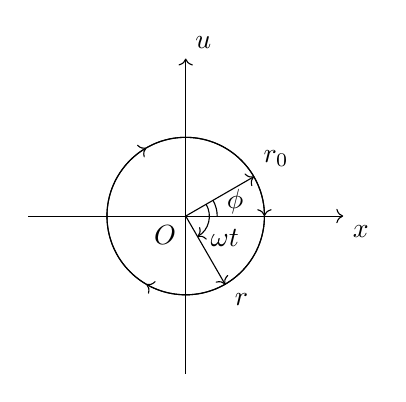
\begin{tikzpicture}
    \draw[->] (-2,0) -- (2,0); 
    \draw[->] (0,-2) -- (0,2);
    \draw[->] (0,0) -- (30:1);
    \draw[->] (0,0) -- (-60:1);
    \node[below right] (B) at (2,0) {$x$};
    \node[below right] (E) at (-15:0.2) {$\omega t$};
    \node[above right] (C) at (0,2) {$u$};
    \node[below left] (O) at (0,0) {$O$};
    \node[above right] (D) at (30:1) {$r_0$};
    \node[above right] (G) at (0.4,-0.1) {$\phi$};
    \node[below right] (F) at (-60:1) {$r$};
    \draw (0,0) circle (1cm);
    \draw[->] (240:1) arc [start angle=240, end angle=120, radius=1cm];
    \draw[->] (1,0) arc [start angle=360, end angle=240, radius=1cm];
    \draw[->] (120:1) arc [start angle=120, end angle=0, radius=1cm];
    \draw[->] (30:0.3) arc [start angle=30, end angle=-60, radius=0.3cm];
    \draw (0.4,0) arc [start angle=0, end angle=30, radius=0.4cm];
\end{tikzpicture}
\]
这张图可以称之为相图(phase diagram),上面每一个点代表了粒子的位置-速度组合,就是粒子的一个状态,粒子状态的不断变化就体现为点的不断移动,这样的移动会划出一条轨迹,我们称之为相轨,图上这条相轨是一个半径为$A_0$的圆,粒子的位置矢量从辐角为$\phi$开始顺时针转动,从物理上,转动方向还可以用以下方式判断:例如粒子在第一象限时,$u > 0$时,$\dot{x}>0$,意味着$x$将增大,因此矢量顺时针旋转。
\subsection{平面运动}
这里尤指在极坐标下的运动,这里就在极坐标中求二阶导数
\begin{align}
    r &= \rho e^{\mathrm{i}\theta}\\
    v &= \dot{r} = \dot{\rho}e^{\mathrm{i}\theta}+\mathrm{i}\rho \dot{\theta} e^{\mathrm{i}\theta}\label{eq:v}\\
    a &= \dot{v} = (\ddot{\rho}-\rho \dot{\theta}^2)e^{\mathrm{i}\theta}+\mathrm{i}(\rho \ddot{\theta}+2\dot{\rho} \dot{\theta})e^{\mathrm{i}\theta}\label{eq:ac}
\end{align}
大部分同学其实对这一步并没有什么问题,直接求出
\begin{align*}
    a_r &=\ddot{\rho}-\rho \dot{\theta}^2\\
    a_\theta &= \rho \ddot{\theta}+2\dot{\rho} \dot{\theta}
\end{align*}
当然题目中还允许答题者使用另一种解法,即利用极坐标的Christoffel符号,请允许我花一些时间,说说如何从复数的角度看待极坐标下的Christoffel符号,如果读者赶时间,可以直接跳过这部分,进入下一问的答案与解析

刚刚说了复数到实平面的映射,我们再来说说复数到平面切空间上的映射,我们把$1$和$\mathrm{i}$作为切空间的两个自然基矢,即
\begin{align*}
    1 &\rightarrow\frac{\partial }{\partial x} \\
    \mathrm{i} &\rightarrow \frac{\partial }{\partial y} 
\end{align*}
其实也本该如此,那么我们来观察一下位置矢量$r$的微分
\[\mathrm{d} r = \mathrm{d} x + \mathrm{i} \mathrm{d} y \]
通过上面的映射,有
\[\mathrm{d} r = \frac{\partial }{\partial x}\mathrm{d} x +  \frac{\partial }{\partial y}\mathrm{d} y \]
又在切空间中,坐标变换默认下面等式成立
\[\frac{\partial }{\partial x}\mathrm{d} x +  \frac{\partial }{\partial y}\mathrm{d} y=\frac{\partial }{\partial \rho}\mathrm{d} \rho +  \frac{\partial }{\partial \theta}\mathrm{d} \theta=\mathrm{d} r\]
我们来计算$\mathrm{d} r$
\[\mathrm{d} r = e^{\mathrm{i}\theta}\mathrm{d} \rho+\mathrm{i}\rho  e^{\mathrm{i}\theta}\mathrm{d}\theta\]
所以
\begin{align*}
    \frac{\partial }{\partial \rho} & = e^{\mathrm{i}\theta} = \varepsilon_r \\
    \frac{\partial }{\partial \theta}& = \mathrm{i}\rho  e^{\mathrm{i}\theta} = \varepsilon_\theta
\end{align*}
这一对\(\varepsilon \)是我们所设的极坐标中的一组基\footnote{需要说明的是,这组基是未归一化的,归一化后的基为\[\varepsilon^*_\mu=\begin{bmatrix}e^{\mathrm{i}\theta}\\\mathrm{i} e^{\mathrm{i}\theta}\end{bmatrix}\]微分容易得到\(\mathrm{d}\varepsilon^*_\mu=\mathrm{i} \varepsilon^*_\mu \mathrm{d} \theta\),所以(\ref{eq:a})可以简单地写成\[\mathrm{d}(V^\mu \varepsilon^*_\mu)= \varepsilon^*_\mu(\mathrm{d} V^\mu + V^\mu\mathrm{i}  \mathrm{d} \theta)\]右边括号内部分除以时间微元常写作\[\dot{v}+\omega \times v\]}
\[\varepsilon_\mu =
\begin{bmatrix}
    e^{\mathrm{i}\theta}\\\mathrm{i}\rho  e^{\mathrm{i}\theta}
\end{bmatrix}\]
对于极坐标中某个矢量$V^\mu$,其真实导数一部分来自于矢量本身的变化,另一部分来自于坐标基矢带来的变化,即
\begin{equation}
    \mathrm{d}(V^\mu \varepsilon_\mu)= \varepsilon_\mu\mathrm{d} V^\mu + V^\mu\mathrm{d}\varepsilon_\mu \label{eq:a}
\end{equation}
所以我们来求\(\mathrm{d} \varepsilon_\mu\)
\begin{align*}
    \mathrm{d} \varepsilon_\mu &= \mathrm{d} \begin{bmatrix}
        e^{\mathrm{i}\theta}\\\mathrm{i}\rho  e^{\mathrm{i}\theta}
    \end{bmatrix} \\ 
    &=\begin{bmatrix}
        0\\\mathrm{i}  e^{\mathrm{i}\theta}
    \end{bmatrix} \mathrm{d} \rho+\begin{bmatrix}
        \mathrm{i} e^{\mathrm{i}\theta}\\-\rho  e^{\mathrm{i}\theta}
    \end{bmatrix}\mathrm{d}\theta\\
    &=\begin{bmatrix}0&0\\0&\frac{1}{\rho}\end{bmatrix}\begin{bmatrix}
        e^{\mathrm{i}\theta}\\\mathrm{i}\rho  e^{\mathrm{i}\theta}
    \end{bmatrix}\mathrm{d} \rho+\begin{bmatrix}0&\frac{1}{\rho}\\-\rho&0\end{bmatrix}\begin{bmatrix}
        e^{\mathrm{i}\theta}\\\mathrm{i}\rho  e^{\mathrm{i}\theta}
    \end{bmatrix}\mathrm{d}\theta\\
    &=\begin{bmatrix}0&0\\0&\frac{1}{\rho}\end{bmatrix}\varepsilon_\mu\mathrm{d} \rho+\begin{bmatrix}0&\frac{1}{\rho}\\-\rho&0\end{bmatrix}\varepsilon_\mu\mathrm{d}\theta
\end{align*}
所以
\begin{align*}
    \frac{\partial }{\partial \rho}\varepsilon_\mu&= \partial_\rho\varepsilon_\mu= \begin{bmatrix}0&0\\0&\frac{1}{\rho}\end{bmatrix}\varepsilon_\mu\\
    \frac{\partial }{\partial \theta}\varepsilon_\mu&=\partial_\theta\varepsilon_\mu=\begin{bmatrix}0&\frac{1}{\rho}\\-\rho&0\end{bmatrix}\varepsilon_\mu
\end{align*}
我们这样摆放这两个导数
\[\begin{bmatrix}
    \partial_\rho\varepsilon_\mu & \partial_\theta\varepsilon_\mu \end{bmatrix}= \begin{bmatrix}
        \begin{bmatrix}0&0\\0&-\rho\end{bmatrix}&\begin{bmatrix}0&\frac{1}{\rho}\\\frac{1}{\rho}&0\end{bmatrix}
    \end{bmatrix}\varepsilon_\mu
\]
我们设
\[
    \Gamma^\rho_{\nu \sigma}=\begin{bmatrix}0&0\\0&-\rho\end{bmatrix} ,\Gamma^\theta_{\nu \sigma} = \begin{bmatrix}0&\frac{1}{\rho}\\\frac{1}{\rho}&0\end{bmatrix}
\]
称之为极坐标下的Christoffel符号\\
所以有
\[\partial_\nu \varepsilon_\mu = \Gamma^\sigma_{\nu \mu}\varepsilon_\sigma\]
这里重复\(\sigma\)指标代表求和\\
代入(\ref{eq:a})中,有
\[\mathrm{d}(V^\mu \varepsilon_\mu)= \varepsilon_\mu\mathrm{d} V^\mu + V^\mu\Gamma^\sigma_{\nu \mu}\varepsilon_\sigma\mathrm{d} x^\nu\]
第二项可以交换哑指标\(\sigma\)和\(\mu\),然后我们对时间求导
\[\frac{\mathrm{d}(V^\mu \varepsilon_\mu)}{\mathrm{d} t}= \varepsilon_\mu(\frac{\mathrm{d} V^\mu}{\mathrm{d} t} + V^\sigma\Gamma^\mu_{\nu \sigma}\frac{\mathrm{d} x^\nu}{\mathrm{d} t})\]
右边括号内的部分可以称为\(V^\mu\)的“真导数”,第一项由矢量本身变化导致,第二项由标架的变化所导致,我们将$x^\nu$和$\frac{\mathrm{d} x^\nu}{\mathrm{d} t}$代入,也能得到(\ref{eq:v})式和(\ref{eq:ac})式的结果。
\subsection{电磁正交场}
\[
\begin{tikzpicture}
    \draw[->] (-2,1) -- (2,1); 
    \draw[->] (-2,0) -- (3,0); 
    \draw[->] (-2,-1) -- (2,-1); 
    \draw[->] (0,-2) -- (0,2);
    \node[above left] (A) at (2,1) {$E$};
    \node[below right] (B) at (3,0) {$x$};
    \node[above right] (C) at (0,2) {$y$};
    \node[below right] (O) at (0,0) {$O$};
    \fill (-1,0.5) circle (2pt);
    \fill (-1,-0.5) circle (2pt);
    \fill (1,0.5) circle (2pt);
    \fill (1,-0.5) circle (2pt);
    \node[above left] (A) at (-1,0.5) {$B$};
    \draw[->] (0,0) -- (30:1);
    \node[above left] (O) at (30:1) {$v_0$};
    \node[below right] (O) at (0.33,0.44) {$\theta_0$};
    \draw (0:0.3) arc [start angle=0, end angle=30, radius=0.3cm];
\end{tikzpicture}
\]
在这个体系中,粒子受力为
\[F = q(E - \mathrm{i} v B)\]
加速度不难写出
\[\dot{v}=\frac{q}{m}(E - \mathrm{i} v B)\]
这算是一个简单的线性方程了,我们简单改写一下
\begin{align*}
    \dot{v}&=-\frac{\mathrm{i} qB}{m}(v+\mathrm{i} \frac{E}{B})\\
    &=-\mathrm{i} \omega_0(v+\mathrm{i} u)
\end{align*}
所以
\[\frac{\mathrm{d}}{\mathrm{d} t}(v+\mathrm{i} u) =-\mathrm{i} \omega_0(v+\mathrm{i} u)\]
解出\(v+\mathrm{i} u\)
\begin{equation}
    v+\mathrm{i} u = (v_0 e^{\mathrm{i} \theta_0}+\mathrm{i} u)e^{-\mathrm{i} \omega_0 t} \label{eq:cir}
\end{equation}
进而得到
\[v=v_0 e^{\mathrm{i} (\theta_0- \omega_0 t)}+\mathrm{i} ue^{-\mathrm{i} \omega_0 t}-\mathrm{i} u \]
下面来画\(v\)在复平面的轨迹,从(\ref{eq:cir})可以看出,\(v+\mathrm{i} u\)这个量在复平面上是顺时针以\(\omega\)的角速度旋转的,下图满足了这种情况
\[
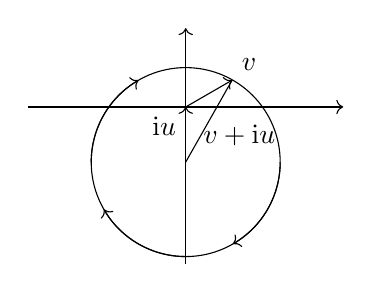
\begin{tikzpicture}
    \draw[->] (-2,0) -- (2,0); 
    \draw[->] (0,-2) -- (0,1);
    \draw[->] (0,0) -- (30:0.68);
    \draw[->] (0,-0.7) -- (0,0);
    \draw (0,-0.7) circle (1.2cm);
    \draw (0,-0.7) -- (30:0.68);
    \node[below left] (O) at (0,0) {$\mathrm{i} u$};
    \node[above right] (A) at (30:0.68) {$v$};
    \node[below right] (B) at (0.1,-0.1) {$v+\mathrm{i} u$};
    \draw[->] (1.2,-0.7) arc [start angle=0, end angle=-60, radius=1.2cm];
    \draw[->] (0,-1.9) arc [start angle=-90, end angle=-150, radius=1.2cm];
    \draw[->] (-1.2,-0.7) arc [start angle=180, end angle=120, radius=1.2cm];
\end{tikzpicture}
\]
这就是\(v\)随t的变化,当\(v_0=0\)时,有
\[v=\mathrm{i} u(e^{-\mathrm{i} \omega_0 t}-1) \]
对其积分,就有
\[r = \frac{u}{\omega_0}(1-e^{-\mathrm{i} \omega_0 t})-\mathrm{i} ut\]
这又是什么样的曲线呢?从表面上看,第一项在旋转,第二项是一个向下的匀速直线运动,为方便起见,我们把\(xOy\)轴逆时针转$90^\circ$,如下图
\[
\begin{tikzpicture}
    \draw[->] (0,-1.5) -- (0,2.3);
    \draw[->] (8,0) -- (-1.5,0); 
    \draw (0,1) circle (1cm);
    \node[below right] (B) at (-2,0) {$y$};
    \node[above right] (C) at (0,2) {$x$};
    \draw[domain=0:8.4,smooth] plot({\x-sin(\x r)},{1-cos(\x r)});
    \draw (4,1) circle (1cm);
    \draw[->] (0,1) -- (0,0);
    \draw[->] (4,1) -- (4.7,1.7);
    \draw[->] (4,1) -- (4.7,1.7);
\end{tikzpicture}
\]
这个图刻画了上面我们求得的结果,另一个物理模型可能会对理解这条曲线有帮助,想象一个轮子静止在原点处,开始向\(y\)轴负方向纯滚,如果我们开始时在轮子最底端做一些标记(例如图上的箭头)那么这一点的在空中划过的轨迹就与上面的轨迹一致\footnote{这一点请读者自证},这条轨迹称为滚轮线或摆线,在本题中,带电粒子似乎在朝着\(y\)轴负方向“漂移”,于是速率\(u=E/B\)也常常称为电漂移速率,有趣的是,这个速率满足
\[\vec{B} \times \vec{u} = \vec{E}\]
\subsection{Kepler运动}
在大质量天体附近,忽略两体效应,万有引力所导致的经典加速度为
\[\dot{v}= -\frac{GM}{\rho^2}e^{i\theta}\]
而且我们还知道有角动量守恒
\[L = \rho^2 \dot{\theta}\]
两式左右相乘,有
\[L\dot{v}=-GM\dot{\theta}e^{i\theta}\]
两边乘\(\mathrm{i}\)移项化简得到
\[\mathrm{d}(iLv+GMe^{i\theta})=0\]
题目给出的初速度为\(\mathrm{i} v_0\)向上,初始\(e^{i\theta}=1\),\(L=v_0\rho_0\)
那么有
\[iLv+GMe^{i\theta}=-Lv_0+GM\]
求得$v$
\[v=iv_0+\frac{\mathrm{i} GM}{v_0\rho_0}(e^{i\theta}-1)\]
通过$v$的不同取值我们有不同的图像与之对应,图中圆的半径为\(\frac{GM}{v_0\rho_0}\),圆心的高度是$(0,v_0)$
\[
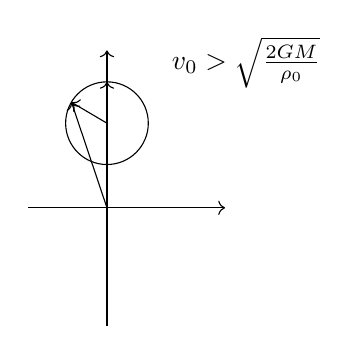
\begin{tikzpicture}
    \draw[->] (-1,0) -- (1.5,0); 
    \draw[->] (0,-1.5) -- (0,2);
    \draw[->] (0,0) -- (0,1.6);
    \draw[->] (0,1.075) -- (-0.45,1.34);
    \draw[->] (0,0) -- (-0.45,1.34);
    \draw (0,1.075) circle (0.525cm);
    \node[above right] (C) at (0.7,1.4) {$v_0>\sqrt{\frac{2GM}{\rho_0}}$};
\end{tikzpicture},
\begin{tikzpicture}
    \draw[->] (-1.5,0) -- (1.5,0); 
    \draw[->] (0,-1.5) -- (0,2);
    \draw[->] (0,0) -- (0,1.4);
    \draw[->] (0,0.7) -- (-0.6,1.05);
    \draw[->] (0,0) -- (-0.6,1.05);
    \draw (0,0.7) circle (0.7cm);
    \node[above right] (C) at (0.7,1.4) {$v_0=\sqrt{\frac{2GM}{\rho_0}}$};
\end{tikzpicture},
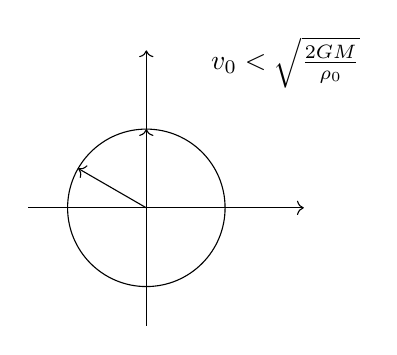
\begin{tikzpicture}
    \draw[->] (-1.5,0) -- (2,0); 
    \draw[->] (0,-1.5) -- (0,2);
    \draw[->] (0,0) -- (0,1);
    \draw[->] (0,0) -- (150:1);
    \draw (0,0) circle (1cm);
    \node[above right] (C) at (0.7,1.4) {$v_0<\sqrt{\frac{2GM}{\rho_0}}$};
\end{tikzpicture}    
\]
这三种情况分别对应三种不同的轨道,只有最右边的才是闭合轨道,所以第一种情形下的相轨不是完整的圆,在下面的一些地方是破缺的;而第二种情况只有一点破缺,这些都留给读者自证

接下来我们代入(\ref{eq:v})式
\[\dot{\rho}e^{\mathrm{i}\theta}+\mathrm{i}\rho \dot{\theta} e^{\mathrm{i}\theta}=\mathrm{i} v_0+\frac{\mathrm{i} GM}{v_0\rho_0}(e^{-\mathrm{i}\theta}-1)\]
利用\(\rho \dot{\theta}=L/\rho\)
我们有
\[-\mathrm{i}\dot{\rho}+ \frac{L}{\rho} =v_0e^{-\mathrm{i} \theta}+\frac{GM}{v_0\rho_0}(1-e^{-\mathrm{i} \theta})\]
选取实部
\[\frac{v_0\rho_0}{\rho}=(v_0-\frac{GM}{v_0\rho_0})\cos\theta+\frac{GM}{v_0\rho_0}\]
于是我们得到
\[\rho(\theta)=\frac{v^2_0\rho^2_0}{GM+(v^2_0\rho_0-GM)\cos\theta}\]
\end{document}